\documentclass[11pt]{article} 

\usepackage{amssymb,amsmath}
\usepackage{graphicx}
\usepackage{caption}
\usepackage{subcaption}
\graphicspath{ {./} }

\newcommand{\numpy}{{\tt numpy}}            % tt font for numpy
\newcommand{\scipy}{{\tt scipy}}            % tt font for scipy
\newcommand{\matplotlib}{{\tt matplotlib}}  % tt font for matplotlib

% \topmargin -1in
% \textheight 9in
% \oddsidemargin  -.25in
% \evensidemargin -.20in
% \textwidth 7in
\topmargin -1in
\textheight 8.5in
\oddsidemargin  -0.25in
\evensidemargin -0.20in
\textwidth 7in

\begin{document}

$$\mbox{\Large \bf CS 111: Homework 8: Due by 11:59 pm Sunday, November 21, 2021}$$
\par\smallskip\noindent
{\bf Submit your paper as one PDF file,
and tell GradeScope which page(s) each problem is on.
If you worked with a partner, 
you must each separately write up and turn in your own homework paper, 
and report the name of your partner.
No groups of more than two.
}

\par\bigskip
{\bf 1.}
The temperature matrix is almost but not quite a Laplacian matrix:
It is symmetric, all its off-diagonal elements are either $0$ or $-1$,
and most of its row sums are $0$.
What's the smallest number of nonzero elements of the
2D temperature matrix with $k=100$ that you would need to change to make 
it into the Laplacian matrix of some graph? 
Which nonzero elements would need to be changed?
Describe in words what graph that is:
How many vertices does it have, and what is the pattern of its edges?

\par\bigskip
{\bf 2.}
The {\em graph partitioning} problem is:
Given an undirected graph $G$ with $n$ vertices, 
divide the vertices into two groups of equal size $n/2$ 
(or, if $n$ is odd, of sizes $(n+1)/2$ and $(n-1)/2$),
with as few edges as possible between vertices in different groups.
Another way to say this is,
color half the vertices red and half the vertices blue while making
the number of edges with one red endpoint and one blue endpoint as small as possible.
Graph partitioning is used in algorithms for parallel computers, 
where you might have two processors cooperating to solve a problem on a big graph;
each processor gets half the graph, 
and the cost of communication between the processors depends on the number
of edges joining the two halves.
The figure below shows two ways to partition a 48-vertex graph,
one cutting 20 edges and one cutting 18 edges.

\begin{figure}[b]
\centering
\begin{minipage}{.5\textwidth}
  \centering
  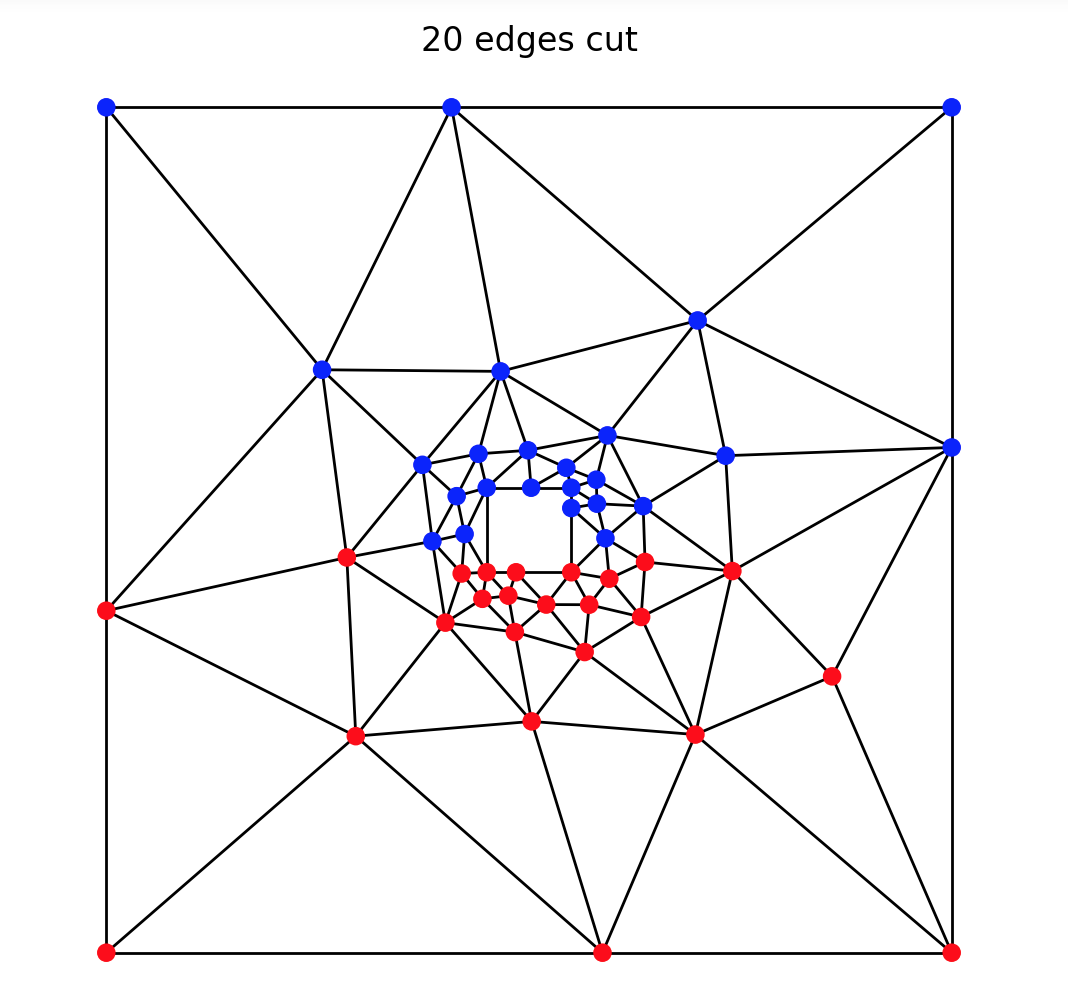
\includegraphics[width=.65\linewidth]{geometric20}
  \captionof{figure}{Geometric partition of 48-vertex graph}
  \label{fig:geometric}
\end{minipage}%
\begin{minipage}{.5\textwidth}
  \centering
  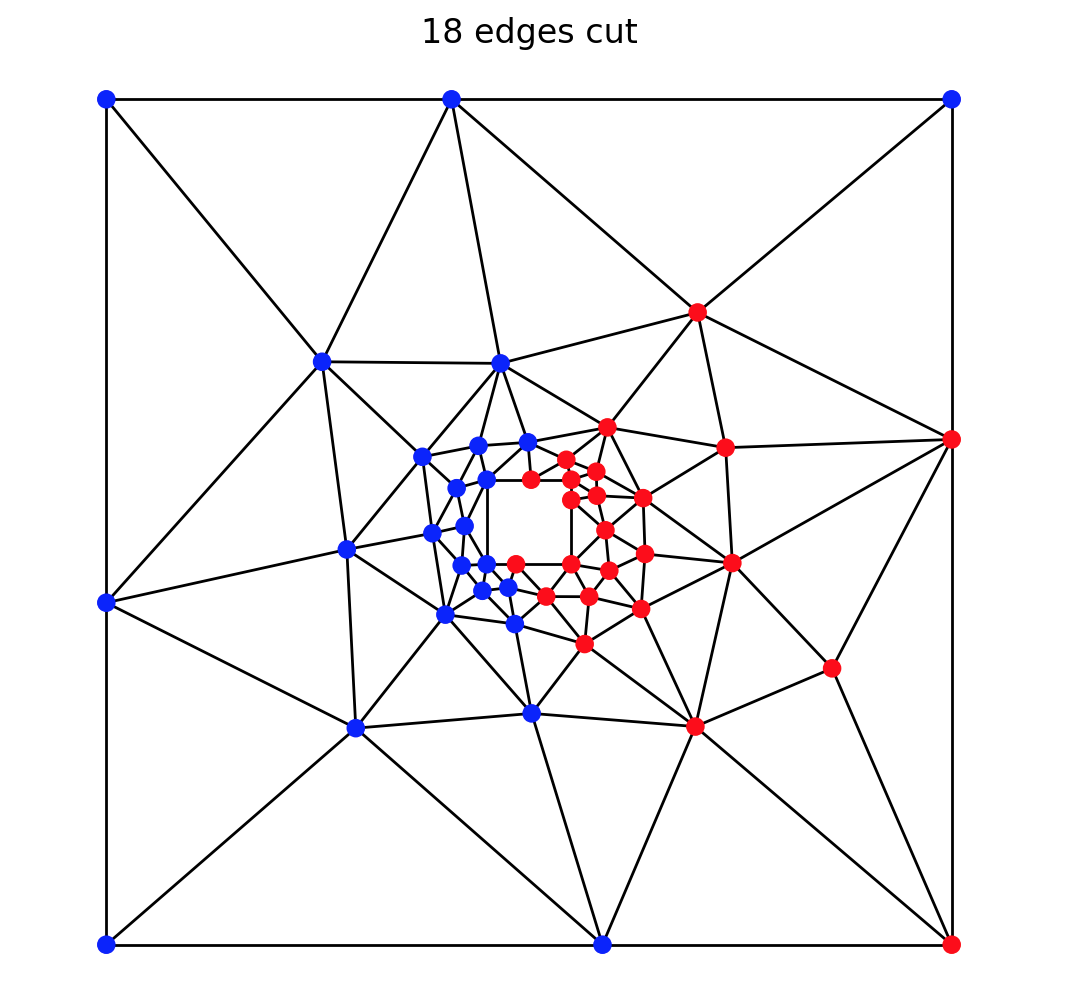
\includegraphics[width=.65\linewidth]{spectral18}
  \captionof{figure}{Spectral partition of 48-vertex graph}
  \label{fig:spectral}
\end{minipage}
\end{figure}

\par\medskip
{\bf 2.1.}
We can describe a partition by labeling each vertex with either a $1$ or a $-1$, 
depending on which part it's in.
Define a {\em cut vector} as an $n$-vector $x$ whose elements are all either $1$ or $-1$.
How many edges cross the cut?
The Laplacian quadratic form $x^TLx$ gives the answer.

Use the formula for the Laplacian quadratic form (which I'll derive in class this week),
$$x^TLx = \sum_{(i,j)\in E}((x(i)-x(j))^2,$$
to prove (give a mathematical argument)
that the number of edges that cross any cut in any graph is equal to
$\alpha \cdot x^TLx$, 
where $L$ is the Laplacian matrix of the graph, 
$x$ is the cut vector,
and $\alpha$ is a fixed constant independent of the graph or the cut. 
What is the value of $\alpha$?

\par\medskip
{\bf 2.2.}
A {\em coordinate cut} is a partition based on a drawing of a graph in the plane,
which colors vertices according to the value of one of their coordinates,
depending on whether the vertex's coordinate is less than or greater than the
median coordinate.
The 20-edge cut in Figure~\ref{fig:geometric} 
is a $y$-coordinate cut of the 48-vertex graph.

Find a $y$-coordinate cut of the airfoil mesh that we saw in class,
make a drawing of it similar to Figure~\ref{fig:geometric}, 
and compute the number of edges that cross the cut by using the Laplacian quadratic form.
(Both the airfoil graph ``airfoil1'' and the 48-vertex graph ``mesh1e1'' are in
the Homework 8 directory on GitHub.
That directory also contains a Jupyter notebook with some helpful routines to
read in graphs in this format and draw them.
You will probably want to use a smaller {\tt node\_size} for the airfoil than 
I did for the 48-vertex graph.)

\par\medskip
{\bf 2.3.}
A {\em spectral cut} is a partition based on the eigenvectors of the Laplacian matrix.
The 18-edge cut in Figure~\ref{fig:spectral} is a spectral cut of the 48-vertex graph.
We'll see in class that the second-smallest eigenvalue $\lambda_1$ is zero if the graph is
not connected.
If the graph is connected, it turns out that
the size of $\lambda_1$ is related to how many edges need to be cut to partition the 
graph, and that the entries in the corresponding eigenvector~$w_1$ can be used to
find a good partition.
(The second eigenvalue and eigenvector of a graph Laplacian, $\lambda_1$ and~$w_1$,
are called the {\em Fiedler value} and the {\em Fiedler vector} of the graph, 
after the mathematician Miroslav Fiedler.)
The idea is similar to a coordinate cut:
Label each vertex with the corresponding element of the Fiedler vector $w_1$,
and choose the part it's in based on whether its label is smaller or larger
than the median element of the Fiedler vector.

Compute the Fiedler value and Fiedler vector for the airfoil graph, 
and use them to find a spectral cut of the airfoil.
Again, make a drawing of it similar to Figure~\ref{fig:spectral}, 
and compute the number of edges that cross the cut by using the Laplacian quadratic form.
(In class this week we'll do an example of computing eigenvalues and eigenvectors 
of the Laplacian matrix of a networkx Graph.)

\end{document}

